\chapter{CellTAN development}

\section{Statistical tests for measure of association} \label{ap1:stats}

\subsection{Pearson's chi squared test} \label{ap1:pearsonschi}

\begin{equation}
    \chi^2 = \sum_{i=1}^{k} \frac{(O_i - E_i)^2}{E_i}
\end{equation}
    
where:
\begin{align*}
\chi^2 & : \text{Chi-squared statistic} \\
O_i & : \text{Observed frequency for category } i \\
E_i & : \text{Expected frequency for category } i \\
k & : \text{Number of categories or cells in the data}
\end{align*}


\subsection{Fischer's exact test} \label{ap1:fischer}

\begin{equation}
    p = \frac{{\binom{a}{x} \binom{b}{y}}}{{\binom{N}{n}}}
\end{equation}

where:
\begin{align*}
    p & : \text{p-value of the test} \\
    a & : \text{Number of successes in group A} \\
    b & : \text{Number of successes in group B} \\
    x & : \text{Number of successes of interest in group A} \\
    y & : \text{Number of successes of interest in group B} \\
    N & : \text{Total number of observations} \\
    n & : \text{Number of observations in group A}
\end{align*}


\subsection{Odds ratio} \label{ap1:oddsratio}

\begin{equation}
OR = \frac{{a \cdot d}}{{b \cdot c}}
\end{equation}

where:
\begin{align*}
OR & : \text{Odds ratio} \\
a & : \text{Number of successes in group A} \\
b & : \text{Number of failures in group A} \\
c & : \text{Number of successes in group B} \\
d & : \text{Number of failures in group B}
\end{align*}

\subsection{Phi coefficient} \label{ap1:phi}

\begin{equation}
\phi = \sqrt{\frac{\chi^2}{N}}
\end{equation}

where:
\begin{align*}
\phi & : \text{Phi coefficient} \\
\chi^2 & : \text{Chi-squared statistic} \\
N & : \text{Total number of observations}
\end{align*}

\subsection{Contingency coefficient C} \label{ap1:contingencyc}

\begin{equation}
C = \sqrt{\frac{\chi^2}{N + \chi^2}}
\end{equation}

where:
\begin{align*}
C & : \text{Contigency coefficient} \\
\chi^2 & : \text{Chi-squared statistic} \\
N & : \text{Total number of observations}
\end{align*}


\subsection{Theil's U} \label{ap1:theilsu}

\begin{equation}
U(x|y) = \frac{H(x) - H(x|y)}{H(x)}
\end{equation}

Entropy of variable x:
\begin{equation}
H(x) = -\sum_{i=1}^{n} p(x_i) \log(p(x_i))
\end{equation}

Conditional entropy of variable x given variable y:
\begin{equation}
H(x|y) = -\sum_{i=1}^{n} \sum_{j=1}^{m} p(x_i, y_j) \log\left(\frac{p(x_i, y_j)}{p(y_j)}\right)
\end{equation}


\section{Technology stack} \label{ap1:techstack}

\begin{figure}[h!]
    \centering
    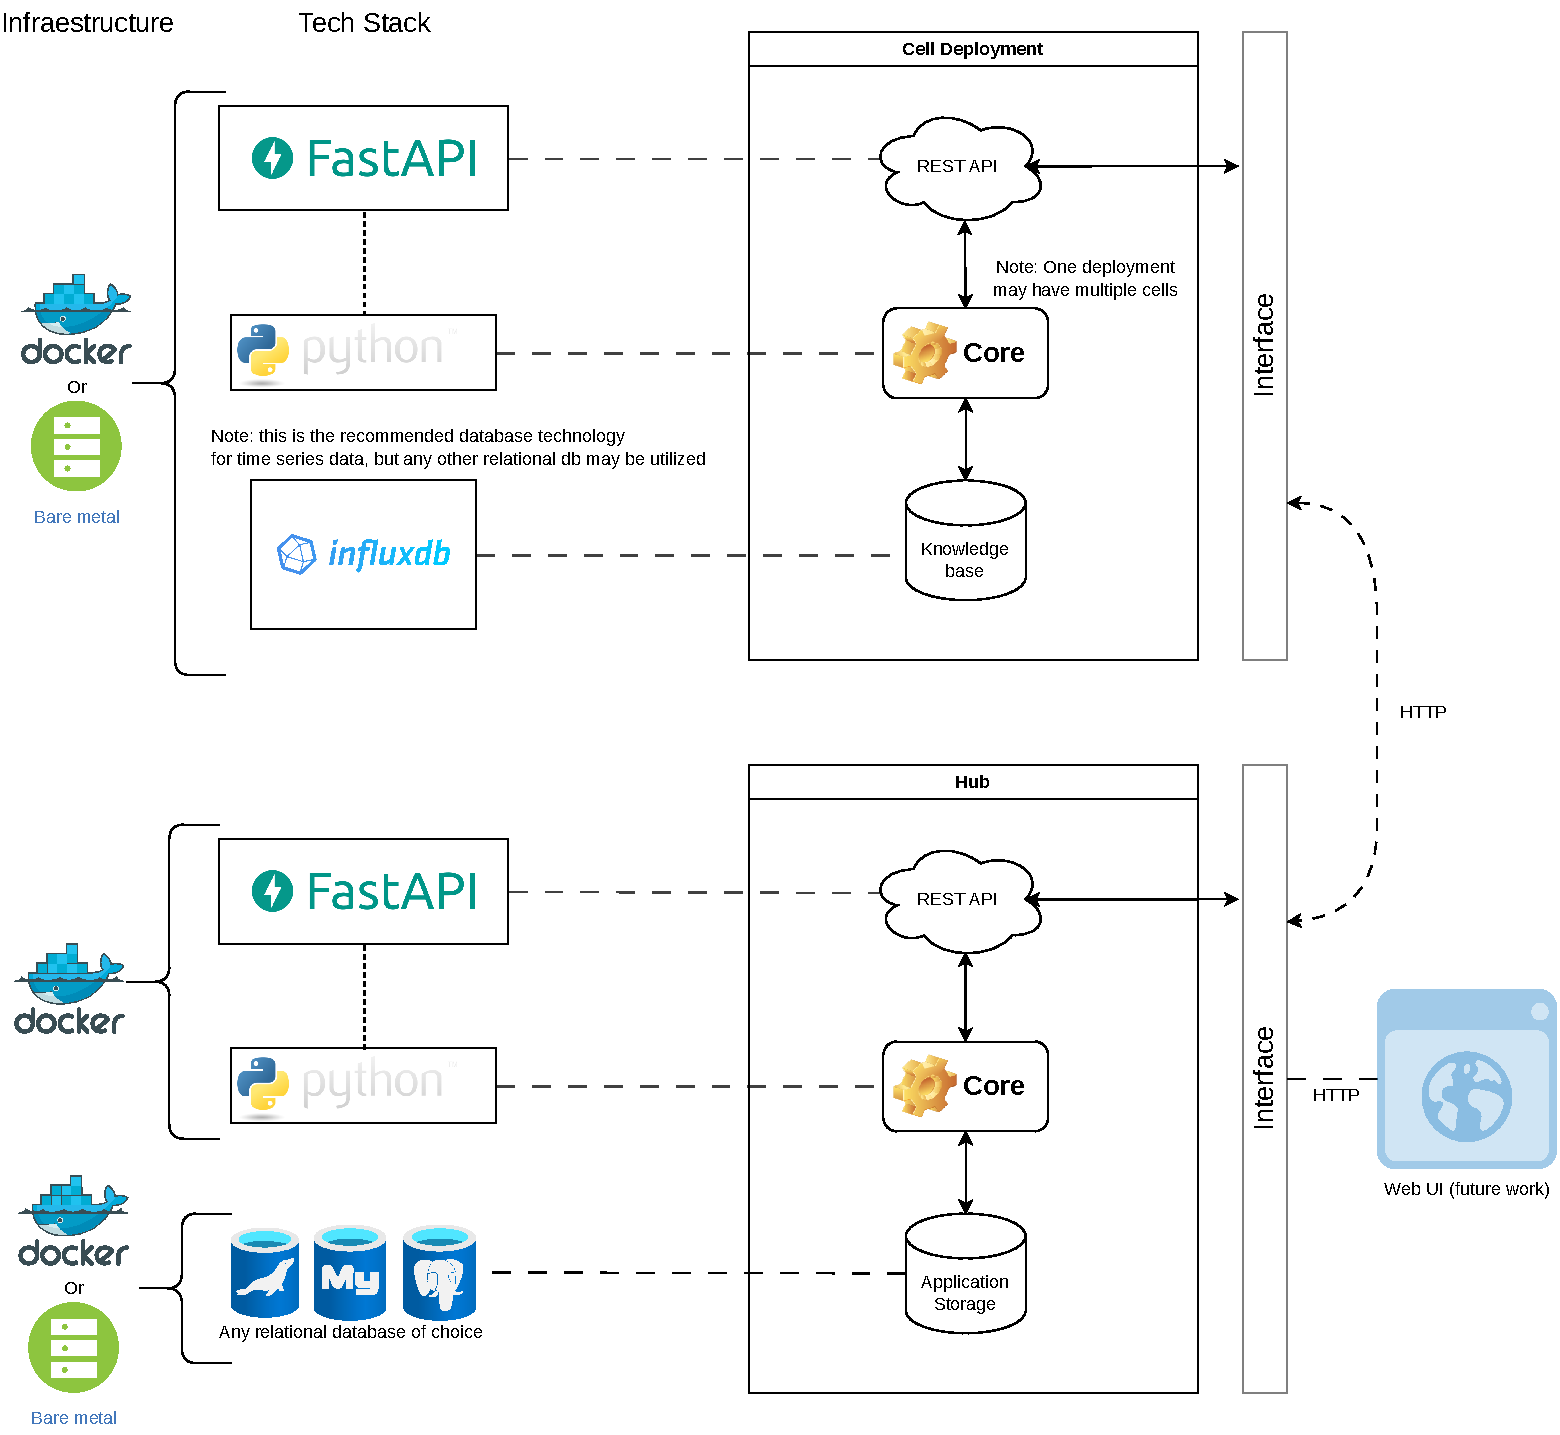
\includegraphics[width=\linewidth]{figures/appendix/techstack.pdf}
    \caption{Technology stack of the Cell and Hub of CellTAN.}
    \label{fig:techstack}
\end{figure}


\section{Cell configuration} \label{ap1:config}
 
% TODO overview da configuração da célula e ficheiro de configuração
